%!TEX root=writeup.tex
\section{Natural Language Based CLI Framework}
\label{sec:framework}

\begin{figure}[h]
    \begin{center} 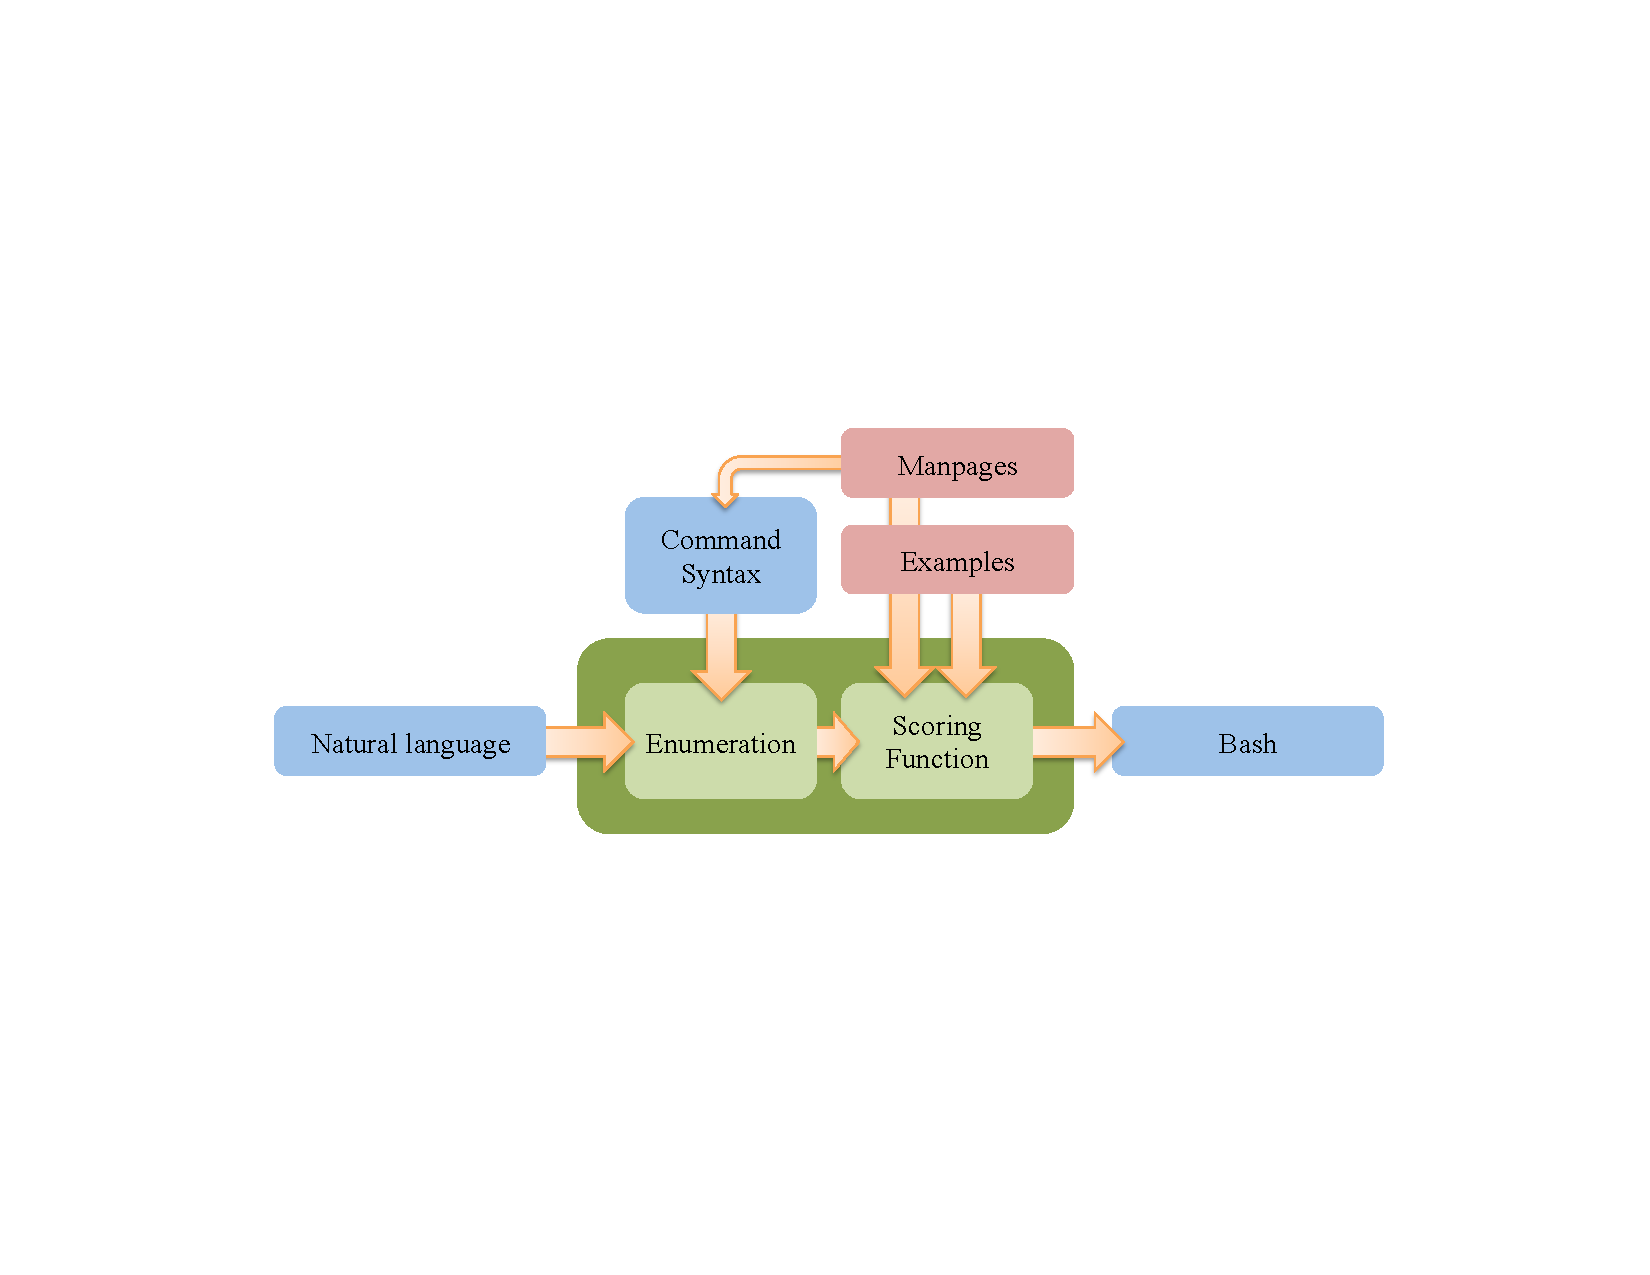
\includegraphics[width=4in]{architecture.pdf} \end{center}
    \caption{The overall architecture of our tool. Offline, the tool learns the
        valid syntax for common Bash commands using manpages. Both the manpages
        and a set of input-output examples are used to learn an appropriate
        scoring function. At runtime, the tool enumerates possible candidate
        programs using the learned syntax, scores them using the learned scoring
        function, and presents the top-ranked suggestions to the user.}
    \label{fig:arch}
\end{figure}

The natural language based command line interpreter we plan to develop consists of two key components: 1) an intermediate language to represent commands and
2) a semantic parser that maps natural language commands issued by users to this intermediate representation. Our initial pilot system is restricted to cover only file system operations, including file lookup, directory tree transformation, file content transformation, and file property modifications. We restrict the domain in the hope that it can be expressed with tractable logic and to reduce the degree of ambiguity in the natural language command. Section~\ref{subsec:represent} introduces the formal language design---the subset of Bash our tool supports---and section~\ref{subsec:parser} introduces the approach to train the semantic parser.

\subsection{Language Design}
\label{subsec:represent}
An ideal intermediate language for the CLI programs should be expressive enough so that it covers many interesting real world cases, and concise enough for the synthesizer to efficiently synthesize. \autoref{fig:lang} presents the syntax of the intermediate language.

\begin{figure}[ht]
\[
\begin{array}{rlll}
\multicolumn{3}{l}{\textbf{Program}}\\
\mathit{p} & :=  & \mathit{cmd}~\overline{\mathit{option}} & \textrm{(Program)}\\
    &  & \mathit{p} ~\|~ \mathsf{xargs} ~\mathit{p} & \textrm{(Pipelined programs)} \\
\mathit{option} & := & \mathit{flag} & \textrm{(Command flag)}\\
                &    & \mathit{val} & \textrm{(Value)}\\
\mathit{cmd} & := & ... & \textrm{(Command names)}\\
\mathit{flag} & := & ... & \textrm{(Flag names)}\\
\mathit{val} & := & ...  & \textrm{(Primitive values)}\\
~\\
\multicolumn{3}{l}{\textbf{Command Signature}}\\
\mathit{sig} & := & \mathit{name}~\mathit{op} & \textrm{(Command signature)}\\
\mathit{op} &:= & \mathit{flag} & \textrm{(Flag)}\\
                &   & \mathit{arg}[\tau] & \textrm{(Argument)}\\
                &   & \mathit{arg}[\tau] ...& \textrm{(Argument list)}\\
                &   & \mathit{op}~|~\mathit{op} & \textrm{(Exclusive options)}\\
                &   & [ \mathit{op} ] & \textrm{(Optional options)}\\
~\\
\multicolumn{3}{l}{\textbf{Rules}}\\
\mathit{rule}^{*} &:=& \mathit{cmd}~\overline{\mathit{option}} : \tau & \textrm{(Command typing rule)}\\
~\\
\multicolumn{3}{l}{\textbf{Types}}\\
\tau_0 & := & \mathsf{void} ~|~ \mathsf{File} ~|~ \mathsf{Date} ~|~ ...& \textrm{(Primitive types)}\\
\tau & := & \tau_0 ~|~ (\bar{\tau}_0)\rightarrow \tau_0 & \textrm{(Type)}
\end{array}
\]
\caption{Intermediate Language syntax, where $\mathit{cmd}$ ranges over strings presernting command names, $\mathit{flag}$ are strings presenting flag names, $\mathit{val}$ presents values in bash programs, and $\mathit{arg}$ represents meta-argument names.}
\label{fig:lang}
\end{figure}


\textbf{Program} defines the formation rules for a program: i.e. a CLI program is either a primitive command or the pipeline of two programs. However, not all of programs that can be represented by the syntax is valid, e.g. the program \code{find -goal} is well formed under the syntax, but it is not a valid real CLI program, as the \code{goal} flag is not part of the command \code{find}. Thus, command signature is introduced to check the well-formedness of a given CLI program. 

The command signature defines the usage of a certain command: a CLI program is well formed only if it follows its corresponding structure. Besides, types help restrict usage of values in a program as other typed languages. Figure~\ref{fig:cmdsig} shows the signature of some commands used in our system. With this signature, a CLI program \code{mv -f -v a.txt b.txt} is will formed as it is captured by the signature of \code{mv}.

\begin{figure}[ht]
\[
\begin{array}{l}

\code{mv [-f | -i | -n] [-v] source:File target:File}\\
\code{mv [-f | -i | -n] [-v] source:File ... directory:File}\\
\code{sort [-bdfgiMnrckmosStTuz] [file:File ...]}\\
\code{grep [-abcdDEFGHhIiJLlmnOopqRSsUVvwxZ] [-A num:Number]} (... rest~omitted)\\
\code{cp [-R [-H | -L | -P]] [-fi | -n] [-apvX] source\_file:File target\_file:File}\\
\code{cp [-R [-H | -L | -P]] [-fi | -n] [-apvX] source\_file:File ... target\_directory:File}\\
\code{ls [-ABCFGHLOPRSTUW\@abcdefghiklmnopqrstuwx1] [file:File ...]}\\
...
\end{array}
\]
\vspace{-15pt}
\caption{Examples of some command signatures.}
\label{fig:cmdsig}
\end{figure}

Since the number of basic Linux commands and options is large even in domain-specific scenarios, it is difficult for a human designer to hand-code all of the generation rules. Though in the course project submission, we create the command signatures by hand, we plan as a longer-term project to semi-automate this step by adding information extracted from the Linux man pages\footnote{\url{http://linux.die.net/man/}}. With this support, extending our tool to handle new commands simply requires adding a new man page to the training data.

\subsection{Natural Language Command Translator}
\label{subsec:parser}
We train the natural language command translator using a set of input/output pairs, each consisting of a natural language query and a command line program, together with manpage descriptions. The online forum StackOverflow has a large volume of input/output pairs. As these conversations are noisy and only a handful of high-quality training pairs can be confidently extracted. On the other hand, Linux man pages are well formatted and contains rich natural language text that explains the usage of each command template and its possible arguments. We propose to use the command-explanation pairs extracted from man pages as additional signals to guide the search for high score rankings, thereby remedies the lack of well-formed training pairs.

We use a linear feature function to score the natural language command to logical representation mappings. The following features are used:
\begin{itemize}\itemsep-1pt
	\item association of key words/phrases to partial expressions
	\item association between partial expressions (e.g. how often do they combined in valid commands)
	\item similarity of key words/phrases in the command to the man page explanation text of a partial expression
	\item complexity of the logical formulas and the commands generated from them.
\end{itemize}
We use the structured perception algorithm to learn weights of the scoring function from the example pairs. In the training process, the input are pairs collected from StackOverflow, and the target is to learn a scoring functions to evaluate the correspondence between the a natural language sentence and a CLI program. In each training iteration, top ranked logical form are selected and the weights are updated based on its similarity to the ground truth logical form. 
% We planned to extend learning into an interactive setting once the basic framework is developed.
